\section{Service Composition}
\subsection{Template}
\begin{figure}[h!]
  \centering
  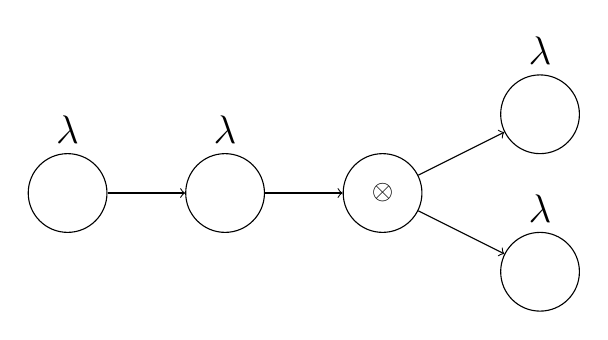
\begin{tikzpicture}
    % Nodes
    \node[draw, circle, minimum size=1cm] (node1) at (0,0) {};
    \node[draw, circle, minimum size=1cm] (node2) at (2,0) {};
    \node[draw, circle, minimum size=1cm] (node3) at (4,0) {$\otimes$};
    \node[draw, circle, minimum size=1cm] (node4) at (6,-1) {};
    \node[draw, circle, minimum size=1cm] (node5) at (6,1) {};

    % Text on top
    \node[above] at (node1.north) {\Large $\lambda$};
    \node[above] at (node2.north) {\Large $\lambda$};
    \node[above] at (node3.north) {};
    \node[above] at (node4.north) {\Large $\lambda$};
    \node[above] at (node5.north) {\Large $\lambda$};

    % Connection
    \draw[->] (node1) -- (node2);
    \draw[->] (node2) -- (node3);
    \draw[->] (node3) -- (node4);
    \draw[->] (node3) -- (node5);
  \end{tikzpicture}
  \caption{Service composition template}
  \label{fig:service_composition_template}
\end{figure}
\textbf{Sequence} ($\oplus$). It composes two service, $wsi$ and $wsj$, in a sequence. $wsi\oplus wsj$ mimics a composition where $wsj$ is executed after $wsi$.

\textbf{Alternative} ($\otimes$). It composes two service, $wsi$ and $wsj$, in an alternative. $wsi\otimes wsj$ mimics a composition where either $wsi$ or $wsj$ is executed.

\textbf{Parallel} ($\oplus$). It composes two service, $wsi$ and $wsj$, in parallel. $wsi\oplus wsj$ mimics a composition where both $wsi$ and $wsj$ are executed simultaneously.

% \textbf{Loop} ($\oslash$). It composes a service composition by iteratively executing the same composition. $\oslash wsi$ mimics a composition where the service $wsi$ is executed a given number of times. In the following, $\oslash$ is considered as a sequence of $\oslash$ services with the same composition $wsi$.

% \textbf{Containment} ($\tau$). It composes two service, $wsi$ and $wsj$, in a containment relation. $wsi\tau wsj$ mimics a basic composition pattern where $wsj$ is called within $wsi$, meaning that $wsi$ assumes the role of a container and $wsj$ uses container-level functionalities (e.g., signature, encryption) to secure the message exchange. We note that the containment operator does not have a direct mapping to BPEL constructs because it is applied to a specific service before the BPEL process is even considered.
\subsection{Instance}
\begin{figure}[H]
  \centering

  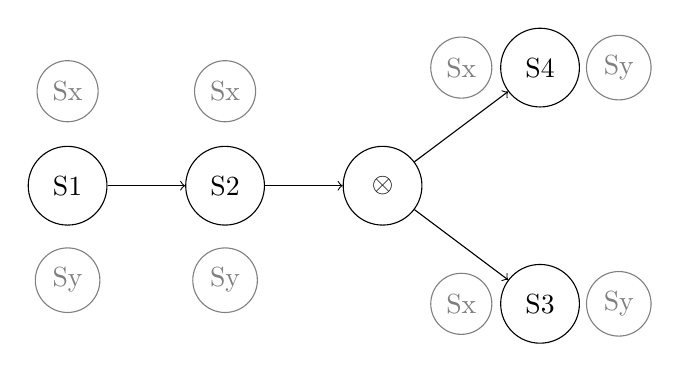
\begin{tikzpicture}
    % Nodes
    \node[draw, circle, minimum size=0.4cm, draw=gray, text opacity=0.5] (node11) at (0,1.2) {Sx};
    \node[draw, circle, minimum size=1cm] (node1) at (0,0) {S1};
    \node[draw, circle, minimum size=0.4cm, draw=gray, text opacity=0.5] (node10) at (0,-1.2) {Sy};

    \node[draw, circle, minimum size=0.4cm, draw=gray, text opacity=0.5] (node22) at (2,1.2) {Sx};
    \node[draw, circle, minimum size=1cm] (node2) at (2,0) {S2};
    \node[draw, circle, minimum size=0.4cm, draw=gray, text opacity=0.5] (node21) at (2,-1.2) {Sy};

    \node[draw, circle, minimum size=1cm] (node3) at (4,0) {$\otimes$};

    \node[draw, circle, minimum size=0.4cm, draw=gray, text opacity=0.5] (node42) at (5,-1.5) {Sx};
    \node[draw, circle, minimum size=1cm] (node4) at (6,-1.5) {S3};
    \node[draw, circle, minimum size=0.4cm, draw=gray, text opacity=0.5] (node41) at (7,-1.5) {Sy};

    \node[draw, circle, minimum size=1cm] (node5) at (6,1.5) {S4};
    \node[draw, circle, minimum size=0.4cm, draw=gray, text opacity=0.5] (node51) at (5,1.5) {Sx};
    \node[draw, circle, minimum size=0.4cm, draw=gray, text opacity=0.5] (node52) at (7,1.5) {Sy};
    % Connection
    \draw[->] (node1) -- (node2);
    \draw[->] (node2) -- (node3);
    \draw[->] (node3) -- (node4);
    \draw[->] (node3) -- (node5);
  \end{tikzpicture}
  \caption{Service composition instance}
  \label{fig:service_composition_instance}
\end{figure}
\[ \forall S \in \mathrm{S}_{C}  \exists  \lambda(S) = \mathrm{S}_{1} \]